\documentclass{article}
\usepackage{graphicx}
\usepackage[UTF8]{ctex}
\usepackage{amsmath}

\title{实验五 组合逻辑电路的设计与测试}
\author{陈岳阳 21级计算机科学与技术}

\begin{document}
\maketitle
\tableofcontents

\newpage
\section{实验目的}
掌握组合逻辑电路的设计与测试方法

\section{实验原理}
1. 使用中、小规模集成电路来设计组合电路是最常见的逻辑电路。设计组合电路的一般步骤如图1所示。

\begin{figure}[htbp]
\centering
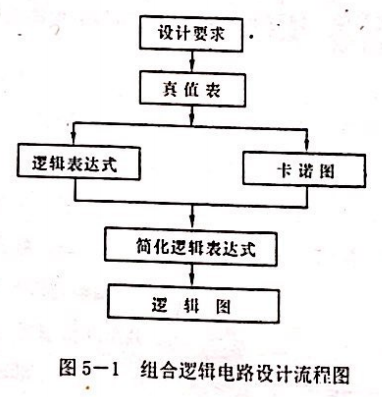
\includegraphics[scale=0.5]{1.png}
\caption{设计流程图}
\label{figure}
\end{figure}

根据设计任务的要求建立输入、输出变量,并列出真值表。然后用逻辑代数或卡诺图化简法求出简化的逻辑表达式。并按实际选用逻辑门的类型修改逻辑表达式。根据简化后的逻辑表达式,画出逻辑图,用标准器件构成逻辑电路。最后,用实验来验证设计的正确性。\\


2.74L554芯片引脚排列

逻辑图如图2

\begin{figure}[htbp]
\centering
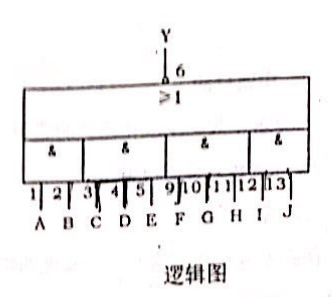
\includegraphics[scale=0.5]{2.png}
\caption{芯片引脚排列逻辑图}
\label{figure}
\end{figure}

\section{设计过程}

~\\
1.逻辑图

本实验中采用的逻辑图如图3

\begin{figure}[htbp]
\centering
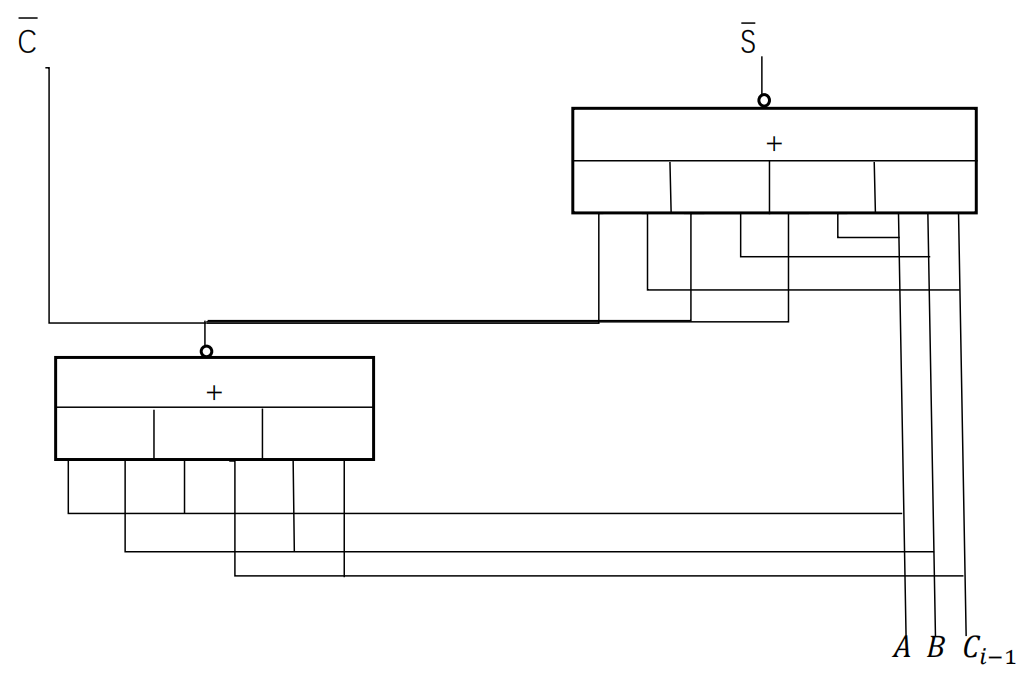
\includegraphics[scale=0.25]{3.png}
\caption{逻辑图}
\label{figure}
\end{figure}

~\\
2.逻辑表达式及化简

$\overline{C}=\overline{AB+AC_{i-1}+BC_{i-1}}=\overline{AB}+\overline{AB}+\overline{AC_{i-1}}+\overline{BC_{i-1}}$

$\overline{S}=\overline{CC_{i-1}+BC+AC+ABC_{i-1}}=\overline{ABC}+\overline{ABC_{i-1}}+\overline{CC_{i-1}}$

~\\
3.真值表

\begin{tabular}{|c|c|c|c|c|}
	\hline
	A&B&$C_{i-1}$&C&S\\
	\hline
	0&0&0&0&0\\
	\hline
	1&0&0&0&1\\
	\hline
	1&0&0&0&1\\
	\hline
	1&1&0&1&0\\
	\hline
	0&0&1&0&1\\
	\hline
	0&1&1&1&0\\
	\hline
	1&0&1&1&0\\
	\hline
	1&1&1&1&1\\
	\hline	
\end{tabular}

\newpage
4.接线图

\begin{figure}[htbp]
\centering
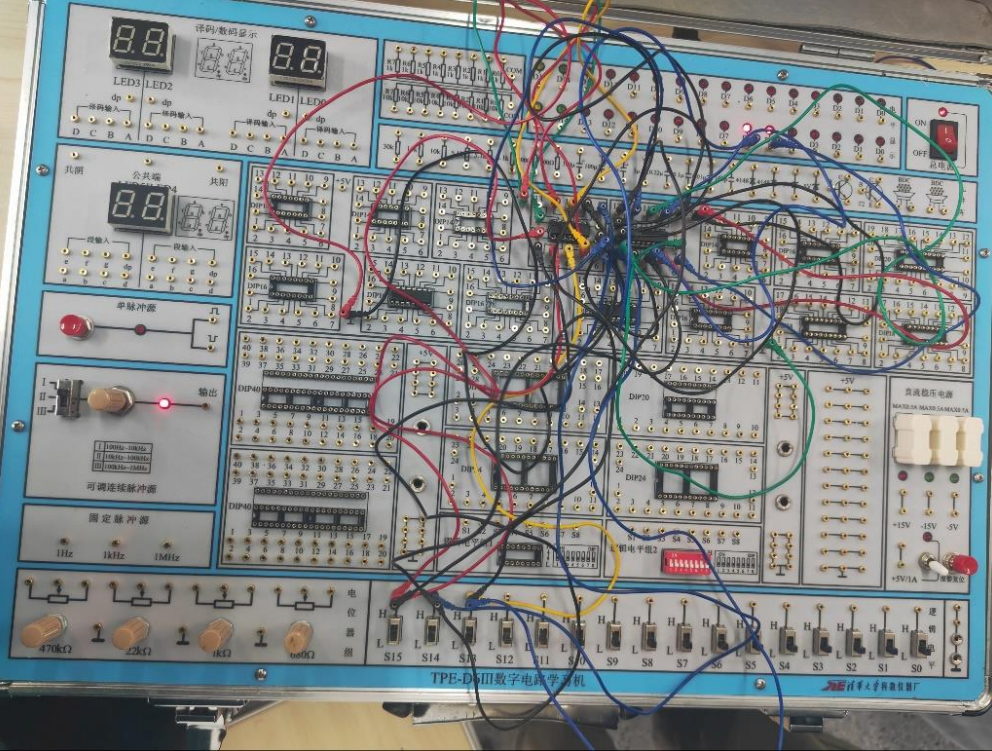
\includegraphics[scale=0.5]{4.png}
\caption{接线图}
\label{figure}
\end{figure}

\section{实验结果}
C端输出连接L1,S端输出连L2,改变输入电压,观察得L1和L2的明亮情况如下:

L1亮的情况:A,B,$C_{i-1}$中至少有两个为低电压时,L1亮。其余情况,L1略微变暗(有明显变化)。

L2亮的情况: $C_{i-1}$为低电压,A、B电压相同;或$C_{i-1}$为高电压,A、B电压不同,L2亮。其余情况,L2暗。

\section{实验总结}

这次实验加深了我对全加器和逻辑电路的理解,深刻记忆了全加器求和与进位规则。同时也增强了动手能力和与同学沟通搭建电路的能力。

\end{document}